%---------------------------------------------------------------------------------------------------------------
% A variation of latex-ninja's simple-hipstercv
% https://github.com/latex-ninja/simple-hipstercv/tree/master
%---------------------------------------------------------------------------------------------------------------



%---------------------------------------------------------------------------------------------------------------
% Imports and a few settings first...
%---------------------------------------------------------------------------------------------------------------

\documentclass[withoutsidebar]{stylishcv} % available options are: darkstylish, lightstylish, withoutsidebar - only lightstylish adjusted to new look from simplehipstercv original, the others may look weirds still

\usepackage[utf8]{inputenc}
\usepackage[default]{raleway}
\usepackage{amsmath}
\usepackage{verbatim}
\usepackage{array}
\usepackage{fontawesome}
\usepackage[most]{tcolorbox}
\usepackage[margin=1cm, a4paper]{geometry}


% A few colors to change them quickly from here without messing with the stylishcv.cls file. Comment/uncomment to change the accent color to your liking, but remember this will overwrite the defaults from darkstylish/lightstylish/withoutsidebar styles!
% 
%\definecolor{accentcolor}{HTML}{FFBA33} %orange
%\definecolor{accentcolor}{HTML}{0094E7} %blue
%\definecolor{accentcolor}{HTML}{FF004F} %red
%\definecolor{accentcolor}{HTML}{30e551} %green
%\definecolor{accentcolor}{HTML}{B32EE1} %purple
%\definecolor{headercolour}{rgb}{0.25,0.25,0.25} %dark grey
%\definecolor{headercolour}{rgb}{0.85,0.85,0.85} %light grey


% Definition of how the rounded section sidebar headers are styled so you can easily change it directly from here
\newtcolorbox{shadedcvbox}[1][]{enhanced jigsaw,
  colback=white!50!headercolour,
  coltext={white},
  boxrule=0pt,
  arc=2mm,
  halign=center,
  auto outer arc,
  boxsep=3pt,
  left=1pt,
  right=1pt,
  bottom=1pt,
  top=1pt,
  fontupper={\scshape},
  #1}


\newtcolorbox{darkshadedcvbox}[1][]{enhanced jigsaw,
  colback=white!0!headercolour,
  coltext={white},
  boxrule=0pt,
  arc=2mm,
  halign=center,
  auto outer arc,
  boxsep=3pt,
  left=1pt,
  right=1pt,
  bottom=1pt,
  top=1pt,
  fontupper={\scshape},
  #1}


% Use this to modify the width of the sidebar and the main part of the page if you need more or less space somewhere. 
\newlength{\rightcolwidth}
\newlength{\leftcolwidth}
\setlength{\leftcolwidth}{0.23\textwidth}
\setlength{\rightcolwidth}{0.75\textwidth}



%---------------------------------------------------------------------------------------------------------------
% Begin document
%---------------------------------------------------------------------------------------------------------------
\begin{document}

	%===========================================================================================================
	% Comment/uncomment to exclude/include a cover letter to your CV. 
	% Write the cover letter in Letter.tex.
	%===========================================================================================================

	\include{Letter\_withoutsidebar}


	% Note: after certain changes, this header seemingly breaks when running pdflatex and looks weird - running it a second time will fix it again =)
	\simpleheader{headercolour}{Olivia}{Owl}{Eagle Owl | Professional Office Bird | Coffee Addict}{accentcolor}

	
	
	
		%===========================================================================================================
		% Picture: you can choose a circle or a square. It will only show uo on the first CV page.
		%===========================================================================================================
		\roundpic{resources/owl.jpg}
		%\squarepic{resources/owl.jpg}

		\vspace{-1.5cm}
		\begin{flushright}
			\begin{minipage}[t]{0.75\textwidth}
				% Other personal information
				\begin{center}
					\begin{shadedcvbox}Personal Information\end{shadedcvbox}
				\end{center}
				% Depending on the length of your text, you may need to adjust coumns widths and spacing a bit to make it look nice again
				\begin{tabular}{L{5cm}  R{8cm}}
					\textbf{Date of Birth}& 01 April 2022\\
					\textbf{Place of Birth} & Mum's Nest\\
					\textbf{Species} & Eagle Owl\\
				\end{tabular}
				\smallskip
			\end{minipage}
		\end{flushright}

		

		% Experience & Skills section. Use the following format for cvevent items: time - Job Position - Company - Location - Description - Image
		\opensectionresume{Experience \& Skills}{0.7}
			\cvevent{05/2023 -- today}{Chief Owl Officer}{The Owl Association}{The Big Tree}{Managing the flock of owls. Still drinking too much coffee.\newline\cvtag{Hiring other owls}\cvtag{Firing other owls}\cvtag{Budget}}{resources/bird-badge.png} \\
			\cvevent{03/2023 -- 04/2023}{Expert Office Owl}{The Owl Association}{The Big Tree}{Drinking too much coffee and staring at other birds at the office\newline\cvtag{Drinking Coffee}\cvtag{Flying}\cvtag{Staring}}{resources/bird-badge.png} \\
			\cvevent{01/2023 -- 02/2023}{Office Owl}{The Owl Association}{The Big Tree}{Brewing coffee for the expert office owls\newline\cvtag{Brewing Coffee and flying it to their desks}\cvtag{Flying}}{resources/bird-badge.png}\\
		\closesection
		\vspace{-0.5cm}

		% Education section. Use the following format for cvdegree items: Title and field of Study - Grade - Institutes - Description - Image
		\opensectionresume{Education}{0.7}
			\cvdegree{09/2022 -- 10/2022}{Flying ~•~Master of Flying (M.Fl.)}{Final grade: 1.0}{University of Birds}{Specialization: Take-Offs\newline Thesis: How to not fall from trees}{resources/institution-icon.png}\\
			\cvdegree{07/2022 -- 08/2022}{Flying~•~Bachelor of Flying (B.Fl.)}{Final grade: 1.0}{University of Birds}{Specialization: Landings\newline Thesis: How to not crash}{resources/institution-icon.png}\\
		\closesection
		
		\begin{minipage}[t]{0.48\textwidth}
			\begin{darkshadedcvbox}Coffee Tasting\end{darkshadedcvbox}
			\begin{tabular}{L{4cm} R{4cm}}
				\textbf{Espresso} & \pictofraction{\faCircle}{accentcolor}{5}{black!30}{0}{\tiny}\\
				\textbf{Latte} & \pictofraction{\faCircle}{accentcolor}{1}{black!30}{4}{\tiny} \\
				\textbf{Cappuccino} & \pictofraction{\faCircle}{accentcolor}{4}{black!30}{1}{\tiny} \\
				\textbf{Americano} & \pictofraction{\faCircle}{accentcolor}{4}{black!30}{1}{\tiny} \\
			\end{tabular}
		\end{minipage}\hfill
		\begin{minipage}[t]{0.48\textwidth}
			\begin{darkshadedcvbox}Flying Skills\end{darkshadedcvbox}
			\begin{tabular}{L{3cm} R{5cm}}
				% "Colored" vs "non-colored" dots should add up to 5: e.g. 5 and 0, 4 and 1, 3 and 2, etc.
				\textbf{Gliding} & \pictofraction{\faCircle}{accentcolor}{5}{black!30}{0}{\tiny}\\
				\textbf{Landing} &  \pictofraction{\faCircle}{accentcolor}{4}{black!30}{1}{\tiny}\\
				\textbf{Take-Offs} &  \pictofraction{\faCircle}{accentcolor}{3}{black!30}{2}{\tiny}\\
			\end{tabular}
			\smallskip
		\end{minipage}
		\smallskip
		
			\simplefooter{headercolour}{white}{
				{\bfseries \scshape Olivia Owl}\\
				\textcolor{accentcolor}{\faMapMarker}~The Nest 1~•~12345 Oak Woods~•~The Forest\\
				{\textcolor{accentcolor}{\faMobile}}~+49~(0)~123 45678~•~
				{\textcolor{accentcolor}{\faEnvelopeO}}~\href{mailto:olivia@owl.com}{olivia@owl.com}\\
				{\textcolor{accentcolor}{\faLinkedinSquare}}~\href{http://linkedin.com}{\texttt{Olivia's LinkedIn}}~•~
				{\textcolor{accentcolor}{\faXingSquare}}~\href{http://xing.de}{\texttt{Olivia's Xing}}~•~
				{\textcolor{accentcolor}{\faGithubSquare}}~\href{https://github.com/}{\texttt{Olivia's Github}}
			}

	%===========================================================================================================
	% Page 2
	%===========================================================================================================
	\switchpage
	\simpleheader{headercolour}{Olivia}{Owl}{Eagle Owl | Professional Office Bird | Coffee Addict}{accentcolor}


	% Certifications sections. Use the following format for cvcertificate items: time - Title and field of course -  Institutes - Certification- Description - Image
	\opensectionresume{Certifications \& Courses}{0.7}
		\cvcertificate{\hspace{1.7cm}08/2023}{Professional Mouse Hunting: Finding Food}{The Bird Association}{Certification: Pro Mouse Hunter}{\cvtag{Hunting}\cvtag{Distinguishing mice and rats}\newline Click on the icon to the right to verify the certificate and badge.}{resources/bird-badge.png}{https://google.com}\\
		\cvcertificate{\hspace{1.7cm}07/2023}{Navigating The Skies}{The Bird Association}{Certification: Pro Owl Pilot}{\cvtag{Flying}\cvtag{Navigation}\newline Click on the icon to the right to verify the certificate and badge.}{resources/bird-badge.png}{https://google.com}\\
		% You can leave the certification
		\cvcertificate{\hspace{1.7cm}07/2023}{Building Nests \& Egg Laying}{The Bird Association}{}{\cvtag{Nesting}\cvtag{Egg Laying}}{resources/bird-badge.png}{https://google.com}\\
	\closesection
	\smallskip
	
		% You can have two sections next to each other by using minipages:
		\begin{minipage}[t]{0.48\textwidth}
			\section*{Olivia's Owl Friends}
			\begin{tabular}{r p{0.6\textwidth} c}
				\cvdegree{Owen}{Nerd Owl}{A geek}{Attending the University of Birds}{}{resources/geekowl.jpg} \\
				\cvdegree{Oscar}{Chef Owl}{Always hungry}{Working at the Grill}{}{resources/chefowl.png} \\
				\cvdegree{Osiris}{Party Owl}{Likes cake}{Runs a bakery}{}{resources/owl-party.png} \\
			\end{tabular}
		\end{minipage}\hfill
		\begin{minipage}[t]{0.48\textwidth}
			% You can use barrule items for example to indicate how strong your programming or language skills are. They are a nice alternative to the colored dots used in the sidebar.
			\section*{Egg Laying Skills}
			\begin{tabular}{r @{\hspace{0.5em}}l}
				\bg{headercolour!30}{white}{Laying Eggs} &  \barrule{0.3}{0.5em}{accentcolor}\\
				\bg{headercolour!30}{white}{Brooding} & \barrule{0.2}{0.5em}{accentcolor} \\
				\bg{headercolour!30}{white}{Caring for Chicks} & \barrule{0.4}{0.5em}{accentcolor} \\
			\end{tabular}
		\end{minipage}
		\smallskip
		
	\begin{minipage}[t]{0.3\textwidth}
			% Languages
			\begin{darkshadedcvbox}Languages\end{darkshadedcvbox}
			\begin{tabular}{l l R{0.75cm}}
				\textbf{Owlish}  & {\phantom{x}\footnotesize Mother Tongue} &\hspace{-0.1cm} C2\\
				\textbf{Birdish} &  \pictofraction{\faCircle}{accentcolor}{4}{black!30}{1}{\tiny} & \hspace{-0.1cm}C1\\
			\end{tabular}
			\smallskip
		\end{minipage}\hfill
		\begin{minipage}[t]{0.15\textwidth}
			%Awards
			\begin{darkshadedcvbox}Awards\end{darkshadedcvbox}
			{\footnotesize
			\begin{center}
				\href{}{\Huge {\color{headercolour}\faInstitution}}\\[\baselineskip]\href{https://google.com}{\bfseries Owl of the Month}
			\end{center}}
			\smallskip
		\end{minipage}\hfill
		\begin{minipage}[t]{0.15\textwidth}
			%Organizations
			\begin{darkshadedcvbox}Organizations\end{darkshadedcvbox}
			{\footnotesize
			\begin{center}
				\href{}{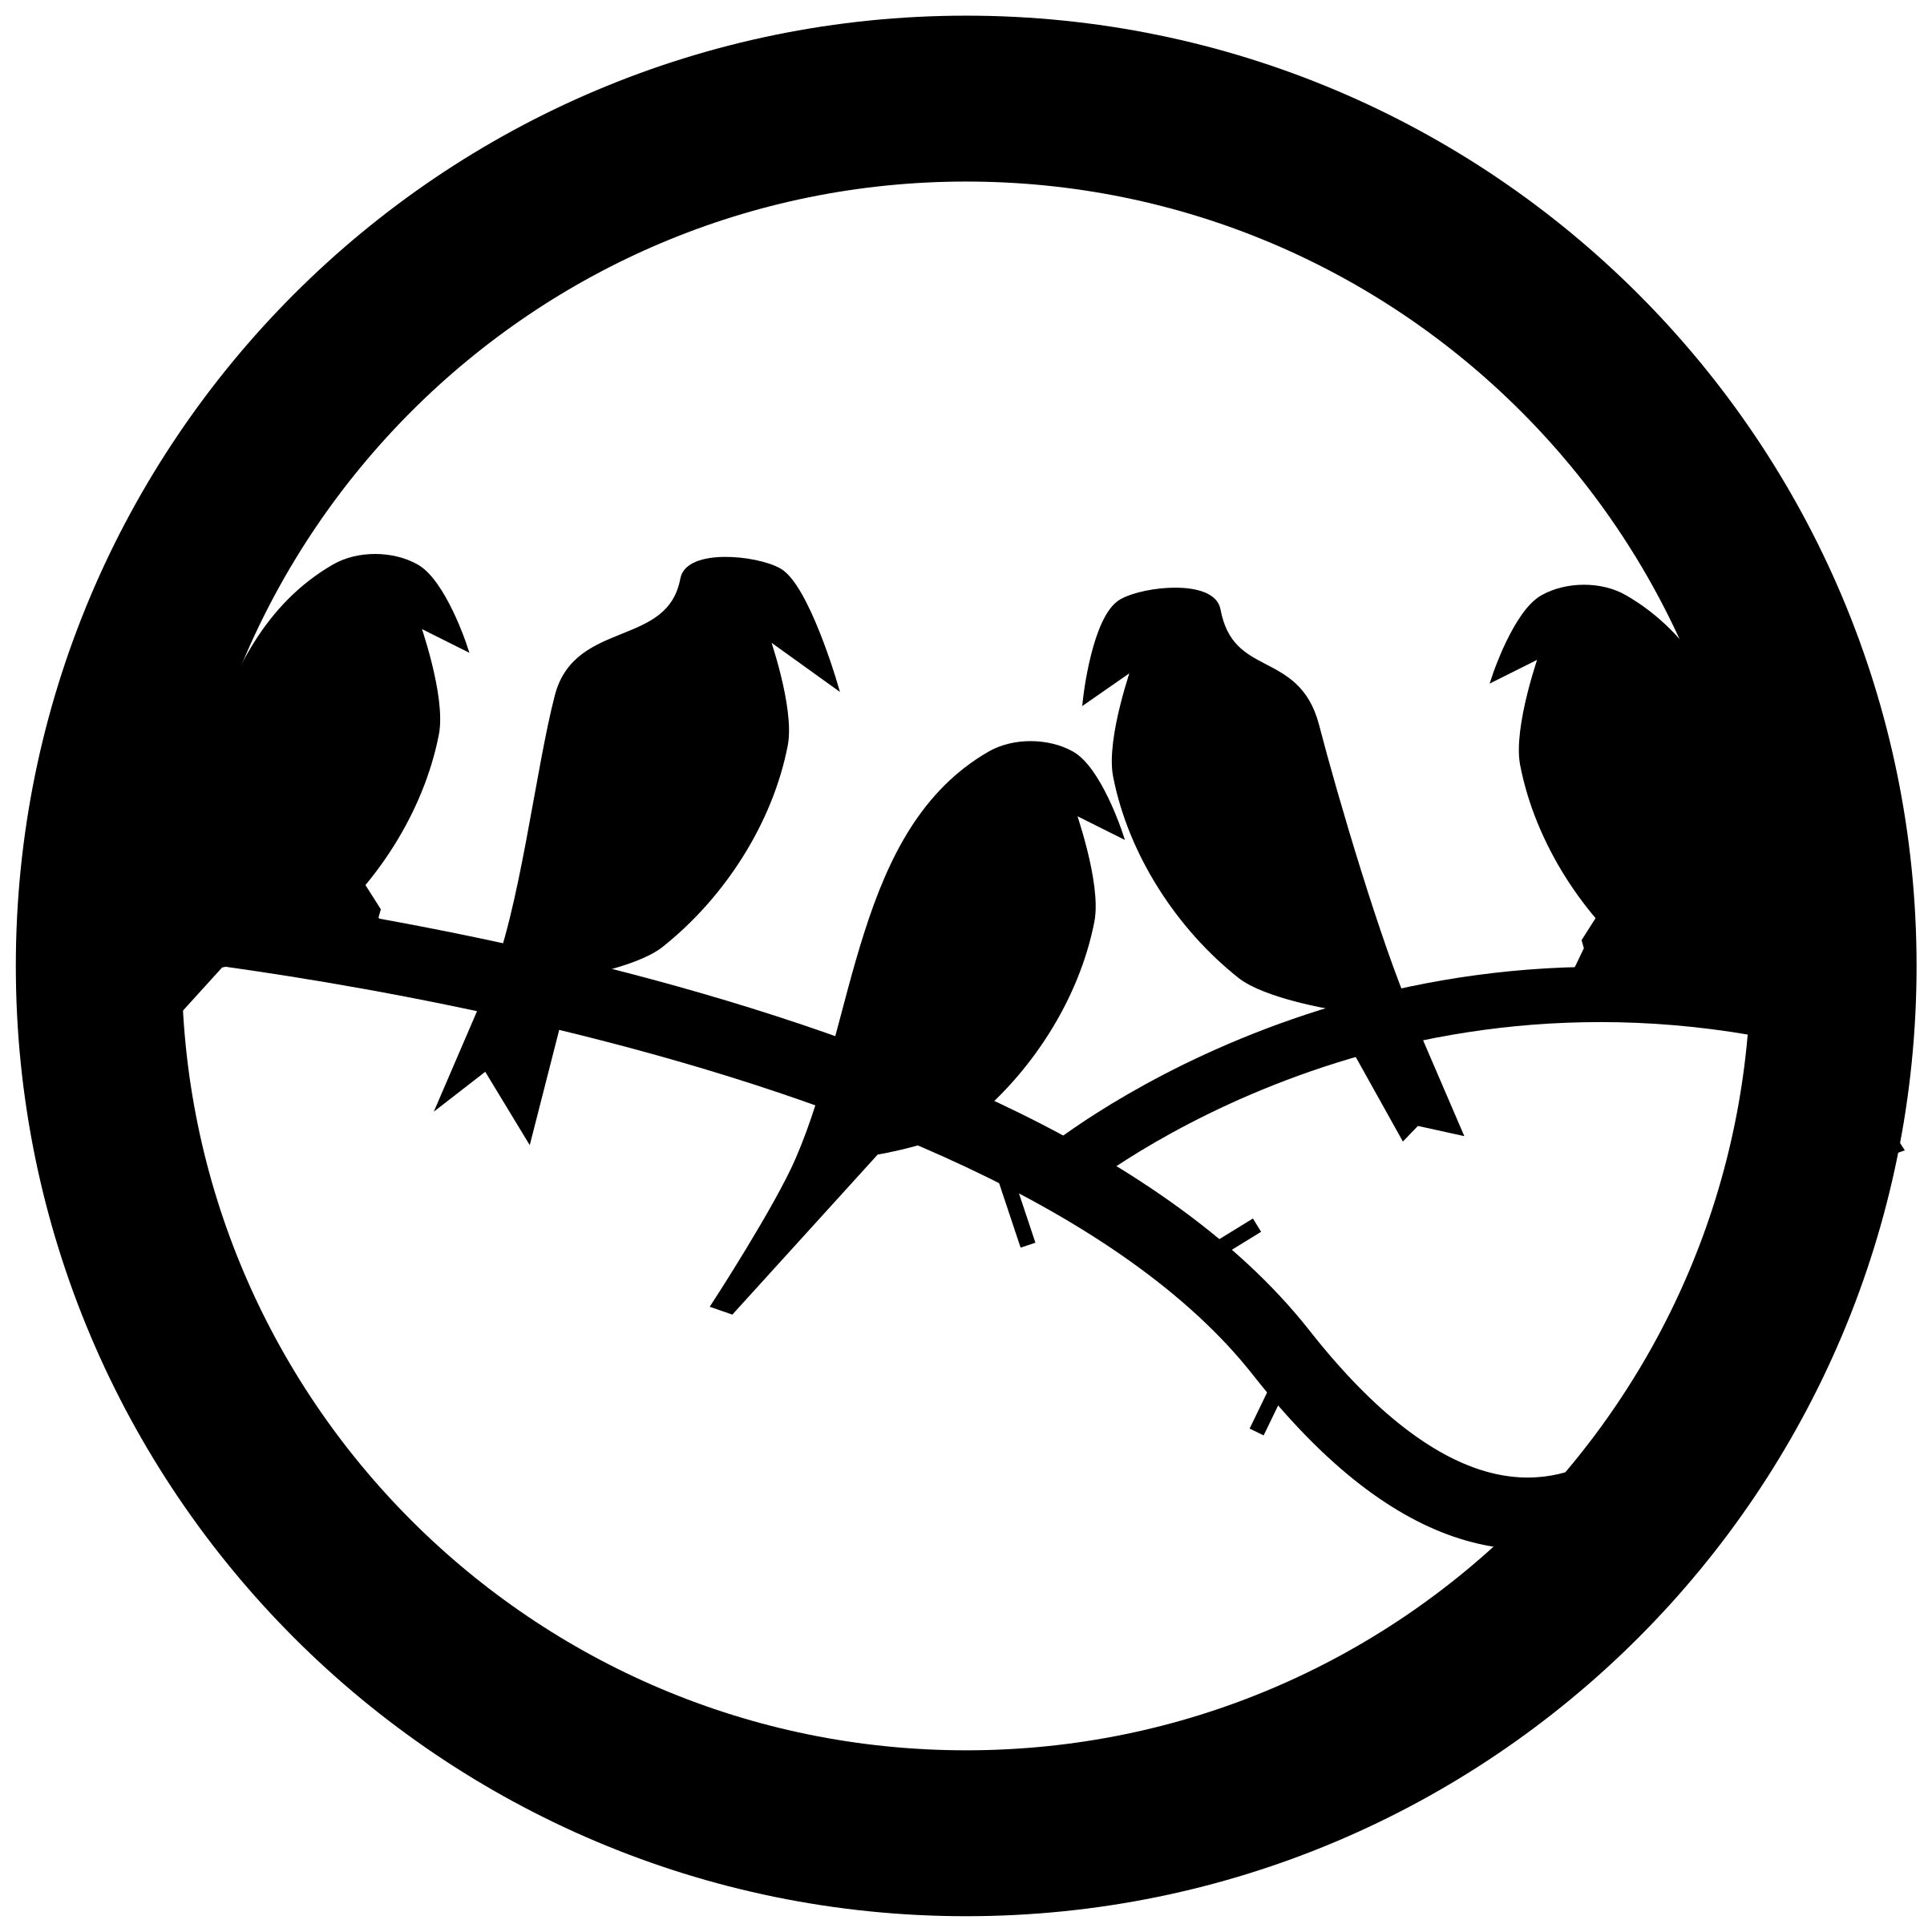
\includegraphics[width=2cm]{resources/bird-badge.png}}\\[\baselineskip]	\href{https://google.com}{\bfseries The Owl Association}
			\end{center}}
			\smallskip
		\end{minipage}\hfill
		\begin{minipage}[t]{0.2\textwidth}
		% Hobbies and hobby icons
			\begin{darkshadedcvbox}Hobbies\end{darkshadedcvbox}
			\begin{center}
				\hobbyicon{\color{iconcolour}\faCoffee}{Coffee}{accentcolor}{\iconsize}{2em}
				\hobbyicon{\color{iconcolour}\faBook}{Books}{headercolour!50}{\iconsize}{2em}\\
				\hobbyicon{\color{iconcolour}\faPlane}{Flying}{headercolour!50}{\iconsize}{2em}
				\hobbyicon{\color{iconcolour}\faTree}{Trees}{accentcolor}{\iconsize}{2em}
			\end{center}
		\end{minipage}
	\bigskip
		

	\begin{minipage}[t]{0.48\textwidth}
		% Another widget you can use for example for contact information
		\begin{darkshadedcvbox}Contact Information\end{darkshadedcvbox}
		\begin{center}
			\scalebox{0.6}{\hspace{-0.3cm}\iconcross{\Huge}{headercolour!30}{accentcolor}%
				{\color{headercolour}\faBook}% top
				{\href{mailto:olivia@owl.com}{\color{headercolour}\faEnvelopeO}}% bottom
				{\color{headercolour}\faPhone}% right
				{\color{headercolour}\faCode} % left
			}
		\end{center}	
	\end{minipage}\hfill
	\begin{minipage}[t]{0.48\textwidth}
		% You can create sections e.g. for specializations, skills, languages, etc.
			\begin{center}
				\begin{darkshadedcvbox}Areas of Specialization\end{darkshadedcvbox}
			\end{center}
			{\footnotesize \begin{center}Flying ~•~ Mouse Hunting ~•~ Staring Contests ~•~ Coffee\end{center}}
			\smallskip
	\end{minipage}
		\vspace{-1cm}

		\simplefooter{headercolour}{white}{
			{\bfseries \scshape Olivia Owl}\\
				\textcolor{accentcolor}{\faMapMarker}~The Nest 1~•~12345 Oak Woods~•~The Forest\\
				{\textcolor{accentcolor}{\faMobile}}~+49~(0)~123 45678~•~
				{\textcolor{accentcolor}{\faEnvelopeO}}~\href{mailto:olivia@owl.com}{olivia@owl.com}\\
				{\textcolor{accentcolor}{\faLinkedinSquare}}~\href{http://linkedin.com}{\texttt{Olivia's LinkedIn}}~•~
				{\textcolor{accentcolor}{\faXingSquare}}~\href{http://xing.de}{\texttt{Olivia's Xing}}~•~
				{\textcolor{accentcolor}{\faGithubSquare}}~\href{https://github.com/}{\texttt{Olivia's Github}}
		}
		
	\resetcolor

	%===========================================================================================================
	% Comment/uncomment to exclude/include any attachments such as references, certificates, etc.
	% Define the atachments you want to include in Attachments.tex.
	%===========================================================================================================
	
	% !TeX root = Main.tex 

\begin{center}

	% Attachment 1
	\simpleheader{headercolour}{Olivia}{Owl}{Eagle Owl | Professional Office Bird | Coffee Addict}{accentcolor}

	% using \centerline inside \begin{flushright} seems weirds, but happens to ensure better spacing to the actual content below.
	\begin{flushleft}\centerline{\large \scshape Olivia's Favorite Picture}\end{flushleft}
	\fbox{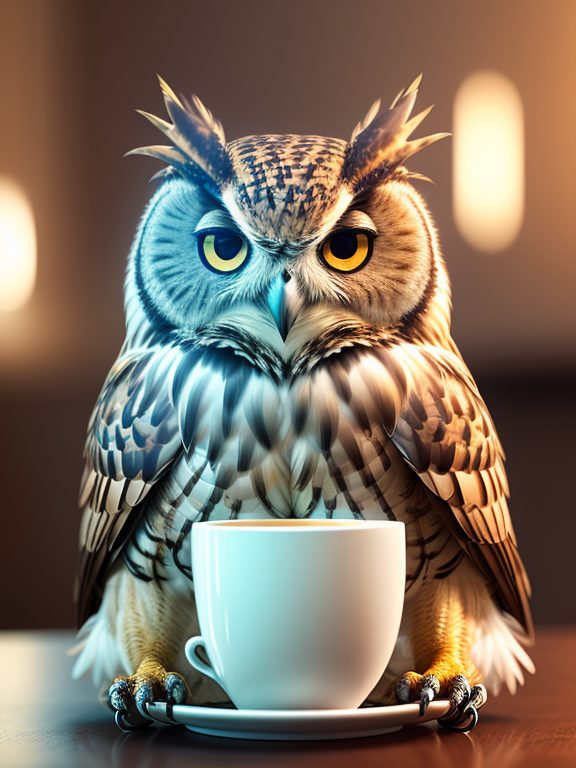
\includegraphics[width=16cm,keepaspectratio,page=1]{resources/fullowl.jpg}}
	\newpage


	% Attachment 2
	\simpleheader{headercolour}{Olivia}{Owl}{Eagle Owl | Professional Office Bird | Coffee Addict}{accentcolor}
	\begin{flushleft}\centerline{\large \scshape Another Portrait of Olivia}\end{flushleft}
	\fbox{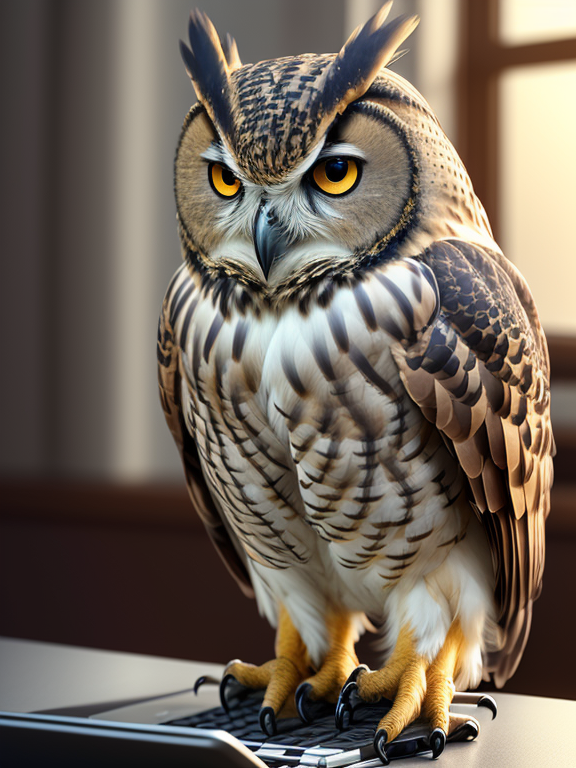
\includegraphics[width=16cm,keepaspectratio,page=1]{resources/fullowl2.jpg}}

\end{center}

\end{document}
